\section{Results}
% ══════════════════════════════════════════════════════════════

\begin{figure*}[t]
  \centering
  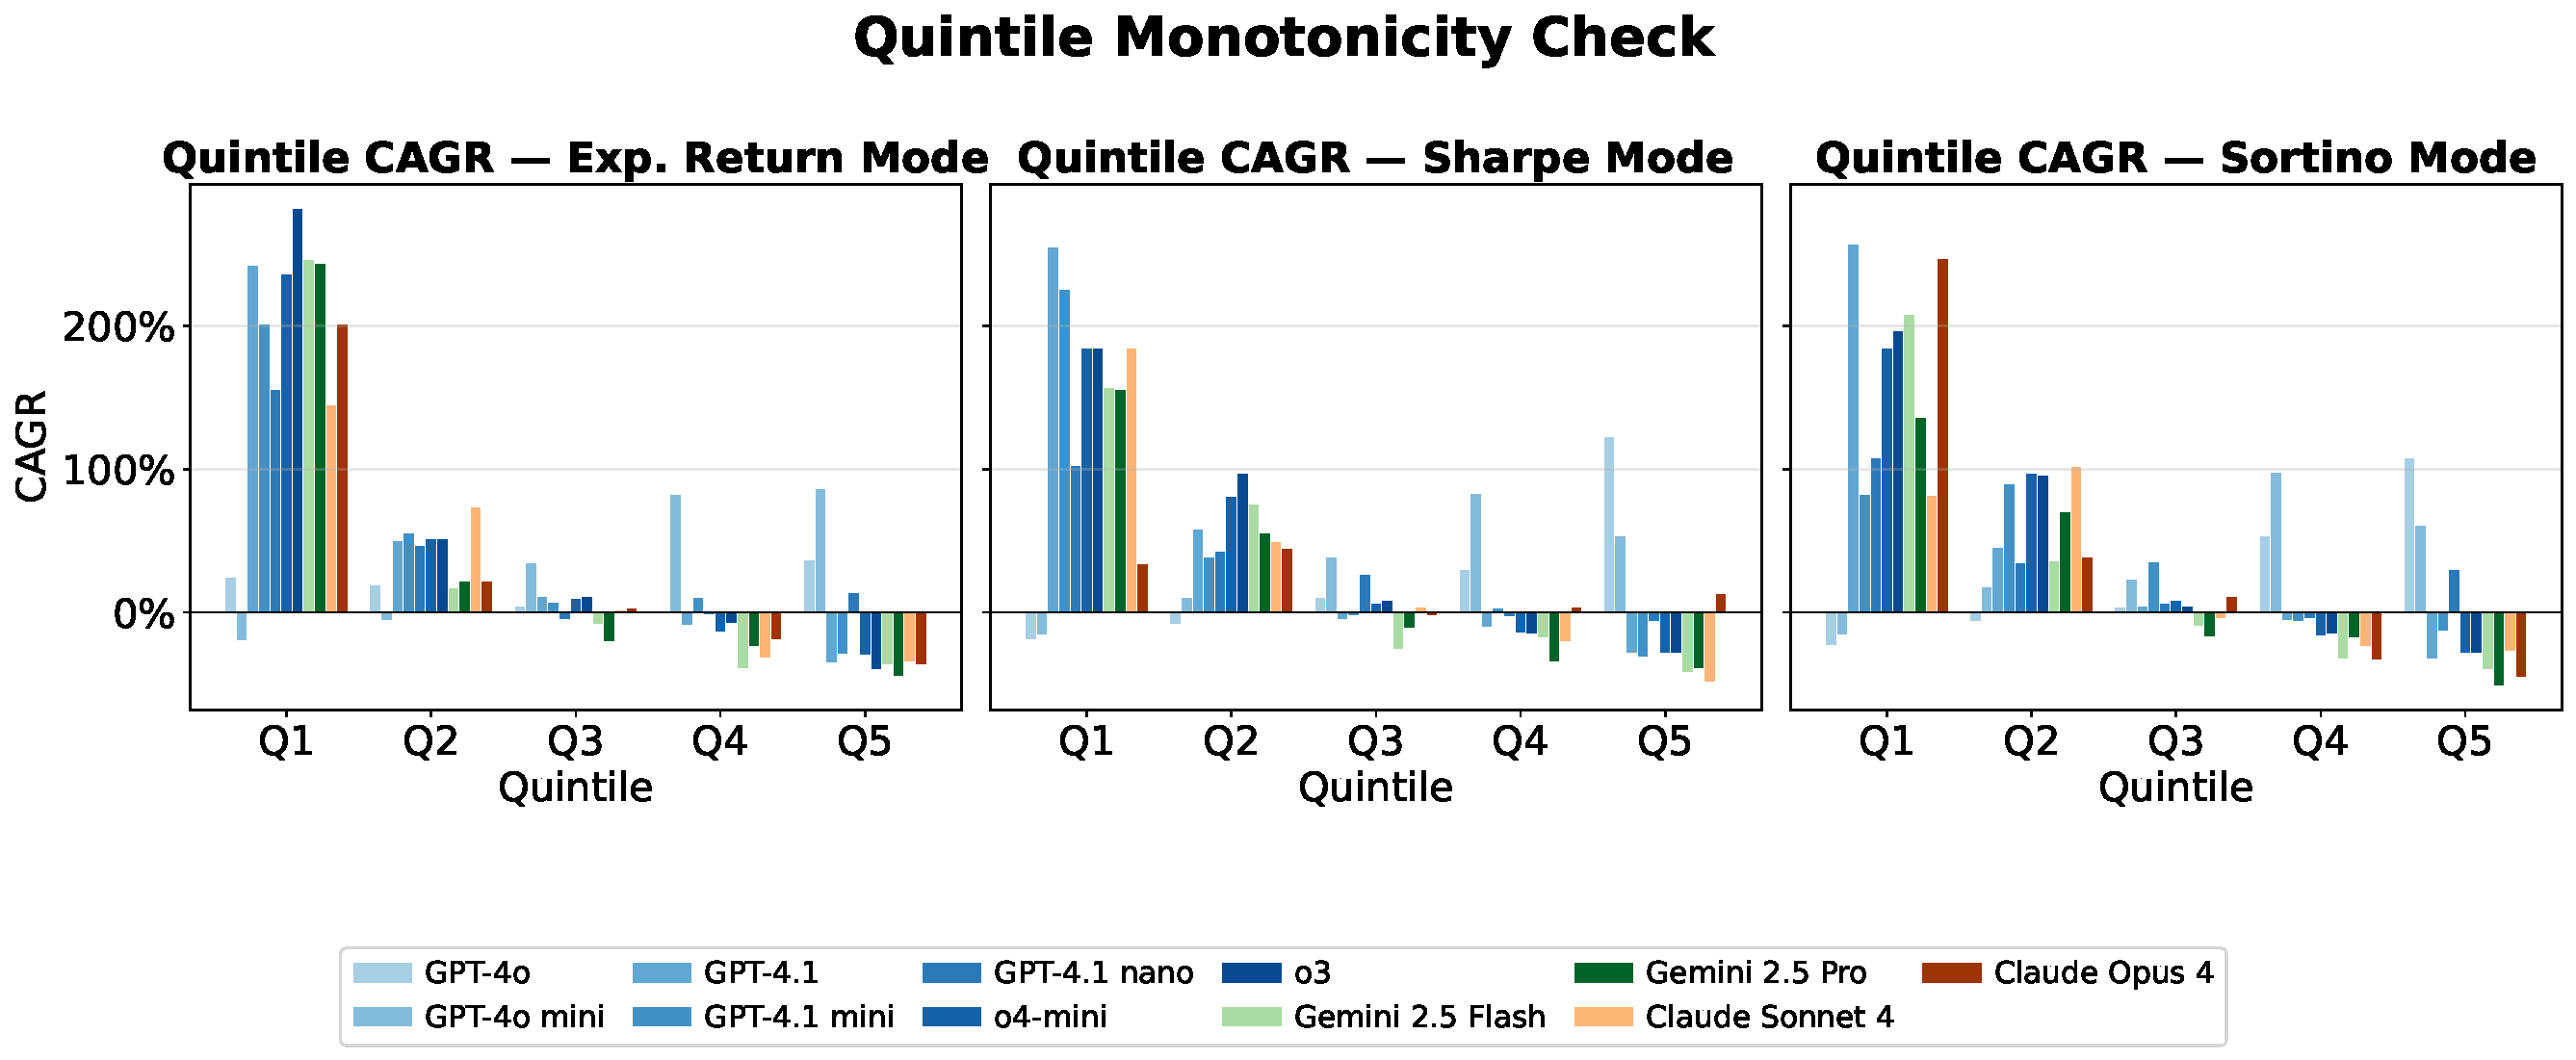
\includegraphics[width=0.95\textwidth]{figures/fig2_quintile_monotonicity.pdf}
  \caption{Quintile CAGR by model and prompt objective in each model's conservative evaluation window.}
  \Description{Grouped bar chart of annualized CAGR across five ranked quintiles for each model and prompt objective, showing strong Q1-to-Q5 separation for o3, Gemini 2.5 models, and GPT-4.1, and reversed patterns for weaker GPT-4o-family models.}
  \label{fig:monotonicity}
\end{figure*}

\subsection{Q1 Performance and Quintile Monotonicity}

Figure~\ref{fig:monotonicity} displays the CAGR of each quintile, the central diagnostic for whether the entire ranking produces cross-sectional separation rather than a single lucky top pick.
\textbf{o3 is the strongest top-quintile ranker}, reaching a Q1 CAGR of 280.4\% (Sharpe = 4.41) in the expected-return mode---far above the benchmarks---with a cleanly monotonic Q1$\to$Q5 pattern.
Gemini 2.5 Flash, Gemini 2.5 Pro, and GPT-4.1 show similarly strong top-quintile performance, with expected-return Q1 CAGRs above 240\%.
In contrast, \textbf{GPT-4o mini produces negative Q1 returns} and negative long--short spreads, a signal worse than random in this evaluation window.
This first screen answers whether the LLM output is an economically ordered ranking at all before applying factor diagnostics.

\subsection{Long--Short Spread}

Table~\ref{tab:longshort} reports the market-neutral Q1$-$Q5 long--short portfolio together with rank IC, with boldface marking the best model within each metric--objective column.
o3 is the strongest expected-return spread model in the conservative window, reaching a 466.0\% net long--short CAGR, Sharpe 5.54, Sortino 10.70, and IC 0.594 after charging both long- and short-leg turnover.
Gemini 2.5 Pro (458.8\%, Sharpe 4.99, IC 0.577), Gemini 2.5 Flash (380.7\%, Sharpe 4.79, IC 0.513), and GPT-4.1 (367.6\%, Sharpe 4.72, IC 0.549) also deliver large positive spreads.
GPT-4o and GPT-4o mini produce negative long--short returns in the conservative window, confirming that model choice can flip the sign of the induced cross-sectional prior.
Because these are annualized short-window portfolio statistics, the relevant evidence is their agreement with IC, ensemble, same-window, and factor-spanning diagnostics, not the CAGR magnitude alone.

\begin{table*}[t]
\centering
\caption{Conservative-window Q1$-$Q5 long--short performance and rank IC, net of 40\,bps one-way costs on both legs. Bold indicates the best value in each column.}
\label{tab:longshort}
\scriptsize
\setlength{\tabcolsep}{1.6pt}
\renewcommand{\arraystretch}{0.95}
\resizebox{0.98\textwidth}{!}{
\begin{tabular}{l rrrrr rrrrr rrrrr}
\toprule
& \multicolumn{5}{c}{\textbf{Exp.\ Return}} & \multicolumn{5}{c}{\textbf{Sharpe}} & \multicolumn{5}{c}{\textbf{Sortino}}  \\
\cmidrule(lr){2-6} \cmidrule(lr){7-11} \cmidrule(lr){12-16}
\textbf{Ranker} & CAGR & Shp & Sort & MDD & IC & CAGR & Shp & Sort & MDD & IC & CAGR & Shp & Sort & MDD & IC  \\
\midrule
GPT-4o & $-$22.7 & $-$0.62 & $-$0.83 & $-$57.3 & 0.090 & $-$70.3 & $-$3.31 & $-$3.89 & $-$86.0 & $-$0.264 & $-$69.8 & $-$3.31 & $-$3.92 & $-$85.7 & $-$0.281 \\
GPT-4o mini & $-$63.1 & $-$4.02 & $-$4.70 & $-$77.0 & $-$0.303 & $-$52.7 & $-$2.92 & $-$3.63 & $-$66.1 & $-$0.241 & $-$55.7 & $-$3.15 & $-$3.86 & $-$69.6 & $-$0.255 \\
GPT-4.1 & 367.6 & 4.72 & 8.37 & $-$11.8 & 0.549 & 342.7 & 4.85 & 9.29 & $-$11.3 & 0.540 & 372.1 & 4.90 & 9.30 & $-$10.8 & 0.510 \\
GPT-4.1 mini & 260.3 & 4.09 & 7.64 & $-$15.9 & 0.449 & 314.0 & 4.82 & 8.96 & $-$8.5 & 0.498 & 81.2 & 2.41 & 4.06 & $-$15.7 & 0.306 \\
GPT-4.1 nano & 100.4 & 2.82 & 4.63 & $-$8.8 & 0.294 & 88.2 & 2.75 & 4.56 & $-$11.6 & 0.300 & 42.1 & 1.80 & 2.71 & $-$8.9 & 0.230 \\
o4-mini & 333.0 & 4.65 & 8.39 & $-$11.4 & 0.529 & 258.7 & 4.48 & 7.75 & $-$8.5 & 0.524 & 258.7 & 4.48 & 7.75 & $-$8.5 & 0.526 \\
o3 & \textbf{466.0} & \textbf{5.54} & \textbf{10.70} & \textbf{$-$8.7} & \textbf{0.594} & 258.7 & 4.48 & 7.75 & $-$8.5 & 0.526 & 274.1 & 4.61 & 8.07 & $-$8.5 & 0.561 \\
\midrule
Gem. 2.5 Flash & 380.7 & 4.79 & 8.81 & $-$14.1 & 0.513 & 298.5 & 4.64 & 8.40 & $-$7.7 & 0.509 & 356.7 & 5.22 & 10.65 & $-$7.1 & 0.482 \\
Gem. 2.5 Pro & 458.8 & 4.99 & 9.15 & $-$11.4 & 0.577 & 270.2 & 4.55 & 8.37 & $-$6.4 & 0.511 & 329.1 & \textbf{5.86} & \textbf{12.38} & \textbf{$-$4.9} & 0.569 \\
\midrule
Cl. Sonnet 4 & 231.9 & 3.99 & 7.24 & $-$9.9 & 0.534 & \textbf{389.3} & \textbf{5.78} & \textbf{11.80} & \textbf{$-$6.0} & \textbf{0.588} & 113.5 & 2.91 & 4.77 & $-$14.8 & 0.539 \\
Cl. Opus 4 & 312.9 & 4.56 & 8.20 & $-$13.0 & 0.483 & $-$1.6 & 0.06 & 0.09 & $-$33.7 & 0.283 & \textbf{444.9} & 5.74 & 11.63 & $-$6.0 & \textbf{0.749} \\
\bottomrule
\end{tabular}
}
\end{table*}


An offline average-rank ensemble check shows that the signal is not purely a single-model artifact.
Table~\ref{tab:ensemble-robustness} averages expected-return ranks across model sets on their common admissible months.
The nine-model consensus across GPT-4.1, o-series, Gemini 2.5, and Claude 4 families reaches a 474.2\% net long--short CAGR, Sharpe 5.44, and IC 0.549 from 2025-07 to 2025-12, while the OpenAI reasoning consensus reaches Sharpe 5.39.

\begin{table}[t]
\centering
\caption{Conservative-window average-rank ensemble robustness. Consensus ranks are evaluated as the same net 40\,bps Q1$-$Q5 portfolio.}
\label{tab:ensemble-robustness}
\resizebox{\columnwidth}{!}{%
\begin{tabular}{lrrrrrr}
\toprule
\textbf{Consensus} & \textbf{Models} & \textbf{Start} & \textbf{Mo.} & \textbf{LS CAGR} & \textbf{LS Shp} & \textbf{IC} \\
\midrule
Nine-model consensus & 9 & 2025-07 & 6 & 474.2 & 5.44 & 0.549 \\
OpenAI 4.1 consensus & 3 & 2025-05 & 8 & 306.8 & 4.49 & 0.486 \\
OpenAI reasoning consensus & 2 & 2025-05 & 8 & 428.9 & 5.39 & 0.567 \\
Gemini 2.5 consensus & 2 & 2025-07 & 6 & 454.2 & 4.86 & 0.542 \\
Claude 4 consensus & 2 & 2025-06 & 7 & 317.2 & 4.57 & 0.560 \\
Low-cost consensus & 3 & 2025-07 & 6 & 379.4 & 4.89 & 0.515 \\
\bottomrule
\end{tabular}
}%
\end{table}


\subsection{Factor Analysis of LLM Rankings}
\label{sec:factor}

The central asset-pricing question is whether LLM-induced orderings behave like factor-like cross-sectional priors.
If rankings simply re-discover known risk premia, their long--short returns should be spanned by standard factor models; if not, they should exhibit distinct loadings and alphas.
We address this with two analyses: (i) time-series \emph{spanning regressions} of Q1$-$Q5 daily returns on established factors \citep{fama1993common,carhart1997persistence,fama2015fivefactor}, and (ii) \emph{characteristic-based style analysis} mirroring the classical factor workflow (sort, form long--short, test alpha) but replacing the human sort with the LLM's ranking.
Section~\ref{sec:input-ablation} applies the same logic to fundamentals-only and market-only input ablations.

\textbf{Spanning test.}
For each expected-return LLM ranker, we regress gross daily Q1$-$Q5 returns on FF6 factors \citep{french2025library} with Newey--West HAC SE (5 lags); Table~\ref{tab:ff6} reports annualized alpha, factor loadings, and adjusted $R^2$.
Three findings stand out: (i) \emph{winning LLMs have large, highly significant alphas}---o3 $\alpha=351\%$ ($t=5.7$), Gemini 2.5 Pro $\alpha=340\%$ ($t=4.7$), and Gemini 2.5 Flash $\alpha=285\%$ ($t=4.7$)---so their returns are not mechanically spanned by the standard factor zoo in this benchmark;
(ii) adjusted $R^2$ ranges from 0.08 to 0.52, indicating that standard factors explain part, but not all, of the spread-return variation;
(iii) \emph{failing models have significantly negative alphas} (GPT-4o mini $\alpha=-55\%$, $t=-4.5$), i.e., structurally counter-factorial during the AI-rally period.

\begin{table*}[!t]
\centering
\caption{FF6 spanning tests for conservative-window Q1$-$Q5 returns. $\alpha$ is annualized percent; stars use Newey--West HAC SE: $^{*}p<0.10$, $^{**}p<0.05$, $^{***}p<0.01$.}
\label{tab:ff6}
\scriptsize
\setlength{\tabcolsep}{2.2pt}
\resizebox{1.5\columnwidth}{!}{
\begin{tabular}{l l r llllll r}
\toprule
\textbf{Model} & $\alpha$ (\%) & $t(\alpha)$ & $\beta_{\text{MKT}}$ & $\beta_{\text{SMB}}$ & $\beta_{\text{HML}}$ & $\beta_{\text{RMW}}$ & $\beta_{\text{CMA}}$ & $\beta_{\text{MOM}}$ & $R^2_{\text{adj}}$  \\
\midrule
GPT-4o & $-$14.2 & $-$0.54 & 0.34$^{***}$ & 0.07 & $-$0.28 & $-$0.03 & $-$0.50$^{*}$ & 0.17 & 0.08 \\
GPT-4o mini & $-$54.8$^{***}$ & $-$4.52 & $-$0.06 & $-$0.14 & 0.21 & 0.07 & 0.58$^{***}$ & $-$0.38$^{***}$ & 0.13 \\
GPT-4.1 & 250.2$^{***}$ & 4.73 & 1.23$^{***}$ & $-$0.48$^{*}$ & $-$0.36 & $-$0.92$^{***}$ & $-$0.23 & 0.36 & 0.45 \\
GPT-4.1 mini & 225.5$^{***}$ & 3.38 & 0.55$^{**}$ & 0.12 & 0.10 & $-$0.61$^{*}$ & $-$0.61 & 0.69$^{**}$ & 0.28 \\
GPT-4.1 nano & 96.6$^{**}$ & 2.39 & 0.74$^{***}$ & $-$0.18 & $-$0.11 & 0.22 & $-$0.39 & $-$0.04 & 0.10 \\
o4-mini & 230.1$^{***}$ & 4.61 & 1.24$^{***}$ & $-$0.45$^{*}$ & $-$0.31 & $-$0.69$^{***}$ & $-$0.42 & 0.32 & 0.44 \\
o3 & 350.8$^{***}$ & 5.71 & 1.15$^{***}$ & $-$0.47$^{*}$ & $-$0.29 & $-$0.67$^{***}$ & $-$0.22 & 0.25 & 0.35 \\
\midrule
Gem. 2.5 Flash & 284.7$^{***}$ & 4.67 & 1.33$^{***}$ & $-$0.32 & $-$0.08 & $-$0.32 & $-$0.54 & 0.58$^{*}$ & 0.48 \\
Gem. 2.5 Pro & 340.2$^{***}$ & 4.71 & 1.49$^{***}$ & $-$0.47 & $-$0.27 & $-$0.48$^{*}$ & $-$0.40 & 0.51 & 0.50 \\
\midrule
Cl. Sonnet 4 & 182.9$^{***}$ & 5.02 & 0.95$^{***}$ & $-$0.46$^{*}$ & $-$0.09 & $-$0.40 & $-$1.02$^{***}$ & 0.45$^{**}$ & 0.52 \\
Cl. Opus 4 & 261.0$^{***}$ & 3.33 & 1.04$^{***}$ & 0.01 & 0.22 & 0.26 & $-$1.39$^{**}$ & 0.12 & 0.25 \\
\bottomrule
\end{tabular}
}
\end{table*}


\textbf{Style fingerprint.}
Because global Fama--French factors are built on the full US cross-section while our universe is 30 mega-cap NASDAQ stocks, they may understate within-universe style tilts.
We therefore rank stocks each month on each characteristic (normalized to $[0,1]$ so that $+1$ is the factor's traditional ``long'' side) and average the rank within each LLM's Q1 and Q5.
Figure~\ref{fig:style} visualizes the Q1$-$Q5 style fingerprint for the expected-return mode.

\begin{figure}[!b]
  \centering
  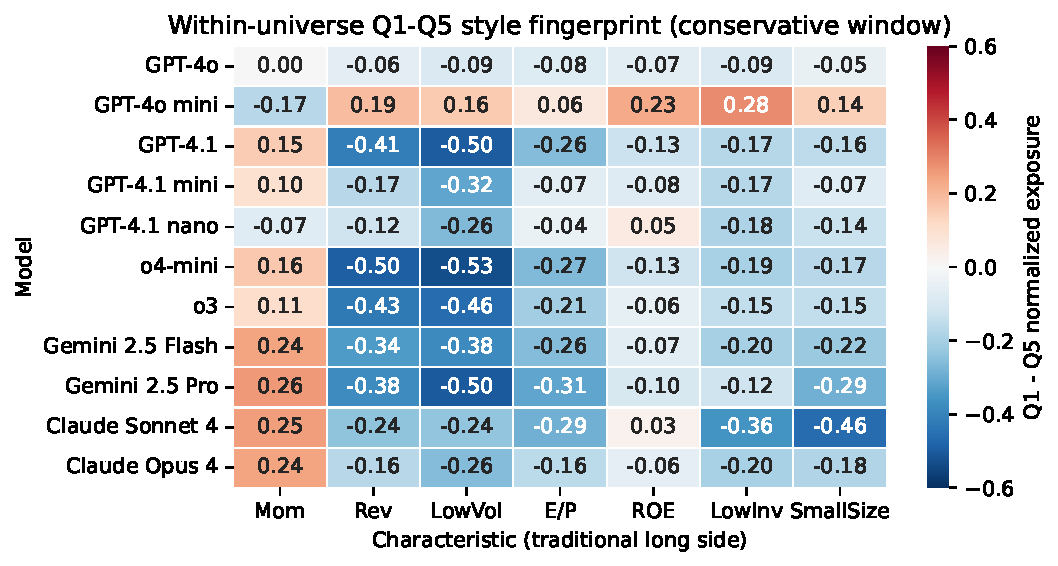
\includegraphics[width=0.96\columnwidth]{figures/fig3_char_fingerprint.pdf}
  \caption{Within-universe Q1$-$Q5 style fingerprint in the expected-return mode. Positive cells tilt toward the characteristic's traditional long side.}
  \Description{Heatmap of characteristic tilts for each model's top-minus-bottom quintile portfolio, with red indicating positive exposure and blue indicating negative exposure.}
  \label{fig:style}
\end{figure}

A consistent pattern emerges across the strongest models: large positive momentum tilts ($+0.23$ to $+0.32$) combined with \emph{negative} exposures to low-volatility, value, profitability, and conservative-investment---a ``growth--momentum chaser'' style that worked in the 2024--2025 AI rally and matches their FF6 loadings in Table~\ref{tab:ff6}.
GPT-4o mini displays the mirror image (negative momentum, positive reversal and volatility), explaining its anti-monotonic returns: it systematically picks defensive, recently-weak stocks in a period when the opposite was rewarded.
Within-universe factor-mimicking correlations show the same qualitative pattern at the daily-return level.

Together these results imply that (a) LLM long--short portfolios in this panel are not fully recovered by linear combinations of classical style factors---consistent with LLM-based factor generation \citep{cheng2024chatgptfactor}---and (b) each LLM embeds a distinct implicit prior over which characteristics predict returns.
Selecting an LLM therefore changes the implicit factor exposure being evaluated.

\subsection{Input Ablation and Factor Loadings}
\label{sec:input-ablation}

The factor-prior interpretation also asks which information channel generates the implicit ranking profile.
We re-run every model--objective pair with fundamentals only, market summaries only, or both inputs, then repeat the FF6 spanning test for one representative model per vendor in expected-return mode.
Table~\ref{tab:input-ablation-main} shows that market-only prompts retain most of the measured signal and slightly exceed the full prompt on average in the conservative window, whereas fundamentals-only prompts are much weaker; Panel C links that performance gap to changes in HML, CMA, and momentum loadings for representative models.
This supports the interpretation that recent market summaries, rather than sparse accounting panels alone, carry most of the observed ranking signal in this narrow universe.

\begin{table}[!t]
\centering
\caption{Input ablation diagnostics under conservative model windows. CAGR and IC are reported in percent; Panel C stars use Newey--West HAC SE: $^{*}p<0.10$, $^{**}p<0.05$, $^{***}p<0.01$.}
\label{tab:input-ablation-main}
\scriptsize
\setlength{\tabcolsep}{3pt}
\resizebox{\columnwidth}{!}{
\begin{tabular}{llrlll}
\toprule
\multicolumn{6}{l}{\textbf{Panel A: Expected-return performance}}  \\
\textbf{Input} & & \textbf{Mean LS CAGR} & \textbf{Mean LS Shp} & \textbf{Mean IC} & \textbf{N}  \\
\midrule
Fund. + Market & & 256.9 & 3.23 & 39.2 & 11 \\
Market only & & 313.8 & 3.38 & 48.7 & 9 \\
Fund. only & & 47.6 & 1.32 & 11.4 & 9 \\
\midrule
\multicolumn{6}{l}{\textbf{Panel B: Paired tests}}  \\
\textbf{Comparison} & \textbf{Metric} & \textbf{Both} & \textbf{Ablated} & \textbf{$\Delta$} & \textbf{$p$}  \\
\midrule
Both - Market & LS CAGR & 218.2 & 294.3 & $-$76.1 & 0.154 \\
Both - Market & LS Shp & 2.68 & 3.21 & $-$0.53 & 0.478 \\
Both - Market & IC & 33.4 & 43.5 & $-$10.1 & 0.154 \\
Both - Fund. & LS CAGR & 218.2 & 20.4 & 197.8 & 0.021 \\
Both - Fund. & LS Shp & 2.68 & 0.53 & 2.15 & 0.096 \\
Both - Fund. & IC & 34.1 & 7.4 & 26.7 & 0.053 \\
\midrule
\multicolumn{6}{l}{\textbf{Panel C: Representative FF6 loadings}}  \\
\textbf{Model} & \textbf{Input} & $\alpha$ & $\beta_{\text{HML}}$ & $\beta_{\text{CMA}}$ & $\beta_{\text{MOM}}$  \\
\midrule
o3 & Fund. + Market & 350.8 & $-$0.29 & $-$0.22 & 0.25 \\
o3 & Market only & 317.4 & $-$0.19 & $-$0.28 & 0.46$^{**}$ \\
o3 & Fund. only & 84.6 & $-$0.50$^{**}$ & $-$0.40 & 0.31 \\
Gem. 2.5 Pro & Fund. + Market & 340.2 & $-$0.27 & $-$0.40 & 0.51 \\
Gem. 2.5 Pro & Market only & 414.2 & $-$0.62 & 0.50 & 0.47 \\
Gem. 2.5 Pro & Fund. only & 76.2 & $-$0.27 & $-$0.69 & 0.38 \\
Cl. Opus 4 & Fund. + Market & 261.0 & 0.22 & $-$1.39$^{**}$ & 0.12 \\
Cl. Opus 4 & Market only & 555.9 & $-$0.20 & $-$0.45 & 0.13 \\
Cl. Opus 4 & Fund. only & $-$7.2 & $-$0.21 & $-$1.26$^{***}$ & 0.18 \\
\bottomrule
\end{tabular}
}
\end{table}


\begin{figure*}[!t]
  \centering
  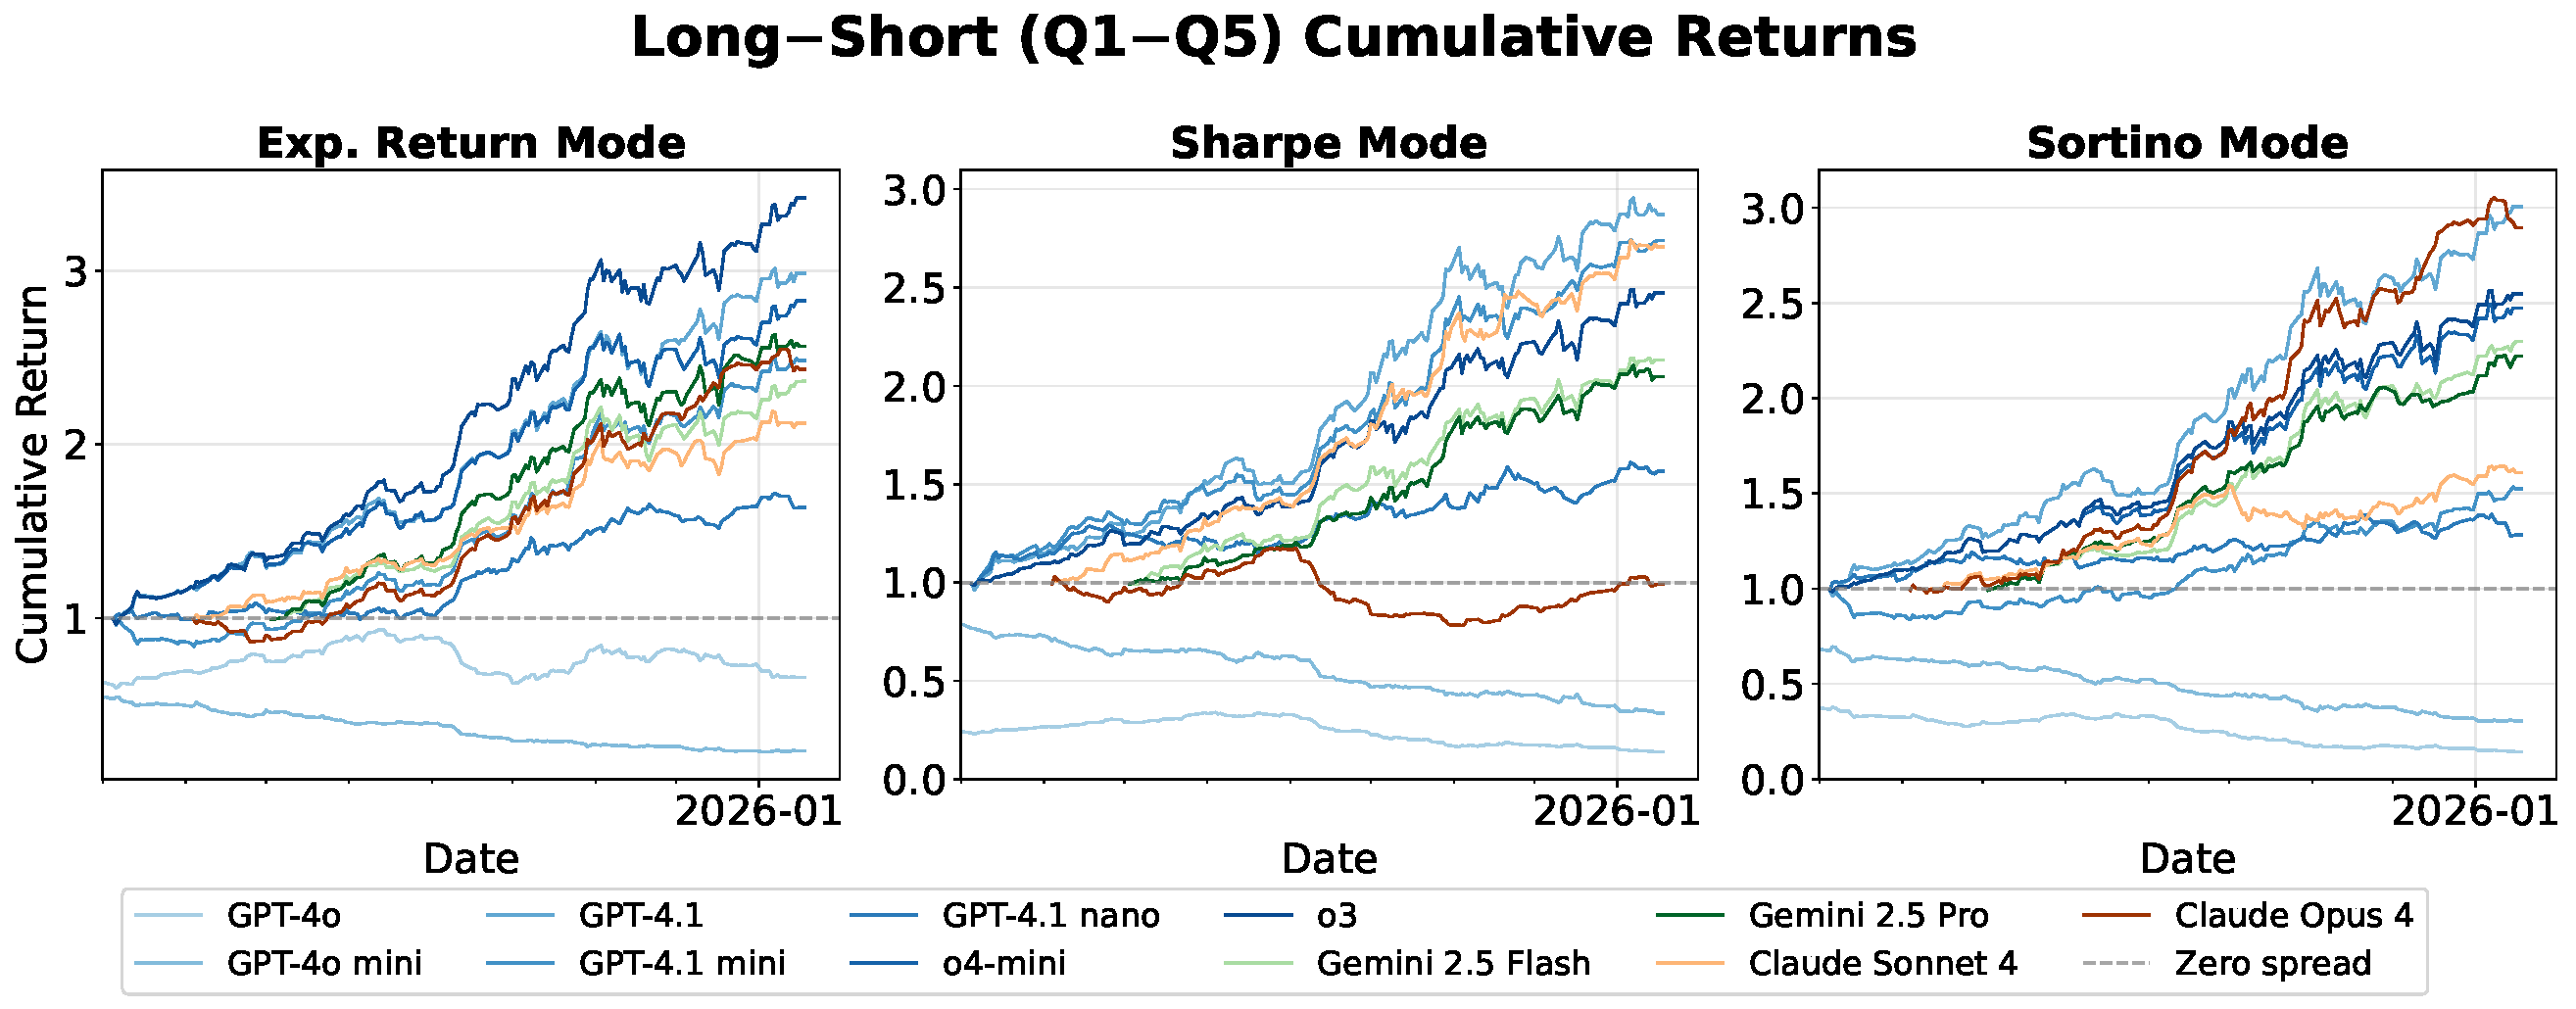
\includegraphics[width=0.94\textwidth]{figures/fig4_ls_cumulative_returns.pdf}
  \caption{Cumulative Q1$-$Q5 wealth by model and prompt objective, shown from 2025-05 after compounding each path from its conservative start; the dashed line marks zero spread wealth.}
  \Description{Line plots of cumulative long-short wealth for each model and prompt objective, displayed from 2025-05 after compounding from each model's conservative start, showing persistent gains for strong models and losses for weak models relative to a zero-spread baseline.}
  \label{fig:ls-cumret-main}
\end{figure*}

\subsection{Rank IC Analysis}

Because Table~\ref{tab:longshort} reports rank IC next to portfolio outcomes, it also checks whether returns arise from genuine cross-sectional ordering rather than a few lucky names.
Across the LLM benchmark, \textbf{o3 achieves the highest expected-return IC} (0.594), followed by Gemini 2.5 Pro (0.577), GPT-4.1 (0.549), and Claude Sonnet 4 (0.534).
GPT-4.1 mini remains positive after patching malformed months (IC = 0.449), while GPT-4o mini is negative across all modes---its rankings are systematically inversely correlated with realized outcomes.

\subsection{Prediction Mode and Cumulative Returns}

Across the included models, the \textbf{expected-return mode remains the clearest primary benchmark}: it directly targets the holding-period objective and produces the strongest spread for several of the top rankers, while Sharpe/Sortino prompts act more like style-control variants.
Sharpe/Sortino prompts win for specific models (e.g., GPT-4.1 reaches its best Q1 CAGR of 257.3\% in Sortino mode) but produce more variable results overall, suggesting expected-return prompts remain the clearest primary benchmark.
Figure~\ref{fig:ls-cumret-main} shows the same pattern in cumulative wealth: the stronger post-2025 rankers, including o3, Gemini 2.5, GPT-4.1-family, and Claude 4 models, accumulate positive spreads, while GPT-4o-family models lose money.

\subsection{Protocol Checks}

Several design choices make the benchmark conservative.
First, all LLM and non-LLM rankers are evaluated on the same monthly universe, holding-period definition, 2-day execution lag, and 40\,bps one-way transaction cost charged to both long- and short-leg turnover.
The performance rows in Table~\ref{tab:longshort} therefore share the same market data, universe, rebalance schedule, and transaction-cost accounting, so differences reflect the induced rankings rather than different portfolio mechanics.
Second, the model table fixes the information boundary induced by knowledge cutoffs.
Because newer models have shorter admissible post-cutoff windows, we avoid interpreting raw CAGR alone and instead emphasize within-vendor generation comparisons, rank IC, same-window non-LLM controls, and FF6 alphas.
The conservative boundary prevents newer preview models from borrowing pre-release 2025 months and makes the negative GPT-4o-family results directly visible.
After patching malformed non-deprecated OpenAI outputs, all included model--mode panels have at least 20 ranked names in each evaluated month.

Third, the listwise protocol uses one deterministic call per model--month--objective rather than prompt search, voting, or hand repair.
Malformed JSON is discarded rather than manually corrected, and temperature is fixed at zero.
This keeps the reported differences attributable to the ranker induced by a frontier model under a common prompt, not to downstream engineering.
It also makes the benchmark a useful lower bound for future agentic systems: an agentic ranker, pairwise tournament, or ensemble should be compared against these single-call listwise results under the same information set and cost accounting.


% ══════════════════════════════════════════════════════════════
